\section{Performance Test Results}
\label{sec:performanceTestResults}
To compare the performance of the two implementations, 
we synthesized each implementation as part of a SoC, programmed the SoCs 
onto the same FPGA boards, and ran 3 types of accelerator applications on the FPGAs. 
Both SoCs have three different accelerators for the three applications: 
Fast Fourier Transform (FFT), General MAtrix Multiply (GEMM), and 2D convolution (CONV2D). 
For each application, we used 5 workload sizes from extra small (XS) to extra large (XL). 
We also tested each application under 2 different coherence modes: LLC-Coherent (Accelerators 
have no L2 cache and only interface with the LLC for coherence) and Coherent (Accelerators 
have L2 caches that are coherent with other L2 caches in processors). While running the applications, 
we measure the number of cycles that the accelerator spends communicating with memory.

\par Figure \ref{fig:dma_chart} shows the speedups calculated from the results of our testing. 
While the speedup for CONV2D stays relatively constant across different workloads, 
the speedup is much larger for FFT and GEMM at smaller to medium workloads. This is 
to be expected, as these workload sizes will allow the accelerators to benefit the most from the improved 
DMA execution of the pipelined LLC. For larger workloads, the accelerators will be primarily receiving 
un-cached data from main memory, so the speedup is not as significant. 


\begin{figure*}[t]
    \centering
    \captionsetup{justification=centering, format=hang}
    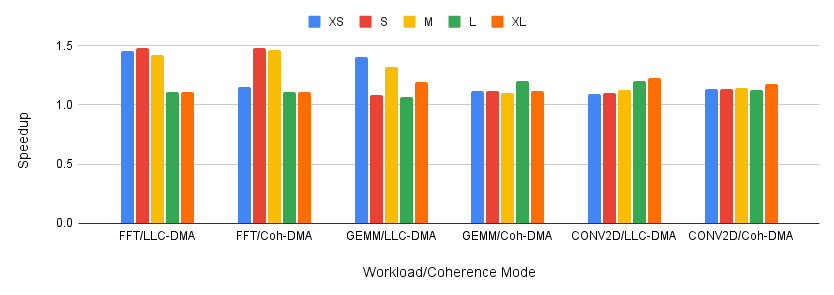
\includegraphics[width=1\textwidth]{fig/DMA_chart.png}
    \caption{Speedup of Pipeline LLC compared to Original LLC for various sizes of applications under different coherence modes. LLC-DMA refers to LLC-Coherent, and Coh-DMA refers to Coherent.}
    \label{fig:dma_chart}
    \end{figure*}
  